%___________________________________________________________________________________________________
\chapter{Series expansion} 



%___________________________________________________________________________________________________
\section{Introduction} 

One of the main focus of numerical methods is to approximate functions by means of different expansions: 

\begin{enumerate} 
\setlength\itemsep{-0.1cm}
	\item Polynomial expansion: Taylor, Lagrange.
	\item Trigonometric series: sine and cosine expansions. 
	\item Expansion by means of known basis: Chebyshev, Legendre, etc. 
\end{enumerate} 

The same function can be expanded or approximated with different basis.
It goes without saying that the computer only allows to sum a finite number $ N $  of terms. 

Hence, the best election is related to the rate of convergence 
of the expansion. In other words, given a tolerance error between the approximation and the exact function, 
the best expansion allows to obtain the approximation with a minimum number of terms $N$. 




%___________________________________________________________________________________________________
\newpage
\section{Expansions of functions} 
   
One of the most used series expansion of a function is its Taylor series, without going any further, in section \ref{sec:intder} we have used a Taylor expansion to estimate the truncation error committed when approximating the derivative of a function by its finite difference expression.

In general, as already mentioned, a series expansion is a very useful way to approximate the value of a given function in a domain. More specifically, the Taylor series, which uses power series, allows us to estimate the value of a function at one point from its value and the value of its derivatives at a different point. Polynomials are extensively known and they are easy to derive, integrate, multiply, etc. so treating a function as its power series approximation can have many advantages when it comes to operating with that function.

A power series of the function $f(x)$ (centered in $x_0 = 0$ and with $N+1$ terms) can be expressed as:
%\[  f(x) = \sum_{k=0} ^N a_k \  x^k, \qquad \qquad a_k = \frac{  f^{(k)} (0)  }{ k! },  \]  
 
\[  f(x) \approx \sum_{k=0} ^N a_k \  x^k,  \] 

where $a_k$ are real numbers that depend only on $k\in \mathbb{N}$ and not on $x$. These coefficients are calculated as:

$$
a_k = \frac{  f^{(k)} (0)  }{ k! }  
$$

being $f^{(k)} (0)$ the \textit{k}-th derivative of $f(x)$ in the point $x_0 = 0$.
 
For a Taylor expansion around a generic point $x_0$ the shape of the polynomial series and the coefficient expressions are:

\[  f(x) \sim \sum_{k=0} ^N a_k \  (x - x_0)^k, \qquad a_k = \frac{  f^{(k)} (x_0)  }{ k! }   \] 





Let's take a look at the Taylor expansion functions proposed here (written with a declarative style). Two approximations are used, one is called under the expected minimum value to be added to the series (epsilon), the other is directly called with the number of terms to be added. Imitating a multilayer structure, previous functions can be recycled, for example \texttt{TaylorE} needs to sum as many terms as the epsilon value requires so the function \texttt{Sigma} function (seen in chapter \ref{sec:Sigma}) is used. In a different way, \texttt{TaylorN} is directly based on \texttt{Sigma\_N} since the number of terms to be added are known and declared as an argument.

Despite that, the structure of both functions is the same, a declaration of the Taylor expansion definition. The \texttt{Sigma} function is called with the general term of the series, the first term to add (which is 0 in this kind of power expansion) and the condition to stop (epsilon value or number of terms). Those are the only ingredients needed to compute the sum series that returns the value of the Taylor expansion in a point $x$. 
  
\vspace{0.5cm}
\renewcommand{\home}{./Fortran/sources/Foundations/Calculus} 
\listings{\home/Taylor_expansions.f90}{function TaylorE}
   {end function}{Taylor_expansions.f90}
   
\renewcommand{\home}{./Fortran/sources/Foundations/Calculus}       
\listings{\home/Taylor_expansions.f90}{function TaylorN}
   {end function}{Taylor_expansions.f90}
   

\newpage   
A couple of details should be noticed here. First of all, the derivatives of the function to be expanded are introduced as an argument in \texttt{Taylor} function. The arguments of this function must be the value where deriving and its order. To do that, a generic procedure is used so it can be recycled next time a function of the same form is used:

$$ 
\myfunc{ \texttt{f\_RxN\_R} }{\mathbb{R} \times\mathbb{Z}}{\mathbb{R}}{\left( x,k \right)}{\texttt{f\_N\_R(x,k)}} 
$$
   
Secondly, both functions are overloaded into one called \texttt{Taylor} so the particularities of each one are transparent for the user, just call a generic function specifying an epsilon value or a number of terms as fourth argument, the calculation is correctly performed automatically. Notice that the \texttt{type} of argument must always be respected so \texttt{N}, the number of terms, must be an \texttt{integer} value and \texttt{eps}, on the contrary, must be a \texttt{real} value.  
   
    
\vspace{0.5cm}   
\renewcommand{\home}{./Fortran/sources/Foundations/Calculus} 
\listings{\home/Taylor_expansions.f90}{interface}
   {end interface}{Taylor_expansions.f90}

\renewcommand{\home}{./Fortran/sources/Foundations/Calculus}  
\listings{\home/Taylor_expansions.f90}{interface Taylor}
         {end interface}{Taylor_expansions.f90}
   

\newpage 
Let's consider the following four examples (included in the Fortran project attached to this book) to better visualize how this function works:

\vspace{0.3cm}
\renewcommand{\home}{./Fortran/sources/Foundations/Calculus} 
\listings{\home/Examples/Series_expansion.f90}{Taylor_expansion_examples}
{contains}{Series_expansion.f90} 

\vspace{-0.2cm}
The first block of code calculates the value of $e$ using a Taylor expansion of the function $e^x$ in $x_0 = 0$. Take a look at the source code to check how the derivative of the function is implemented.  Three calls are performed with $N = 1$, $N = 4$ and $eps = 1e-7$. As it is expected, each result returns a better approximation to the value of $e = 2.7182818284...$:
\begin{verbatim}
Taylor exp(1.) x0=0   :   2.00000000000000
Taylor exp(1.) x0=0   :   2.70833333333333
Taylor exp(1.) x0=0   :   2.71828182619849
\end{verbatim}
   
The other three blocks of code compare some functions with their Taylor series expansions. In the first place a cosine function is compared with its Taylor expansion around $x_0 = 0$ using $N = 10$ (11 terms of the series). The plot shows a black cosine curve in the interval $\left[0,2\pi\right]$ compared with a red curve with its series expansion (figure \ref{fig:Taylor1}). The same, with $N = 5$, is done with the function $f(x) = \frac{1}{1-x}$ in the interval $\left[-2,2\right]$, the result is seen in the the figure \ref{fig:Taylor2}. Finally, the cosine is approximated by 7 different curves, each of them considering more terms of the series expansions ($N = 1, 5, 9, 13, 17, 21$ and $25$) so the result converges to the cosine function (figure \ref{fig:Taylor3}). 

\begin{figure}
    \begin{subfigure}[h]{0.4\textwidth}
        \centering
        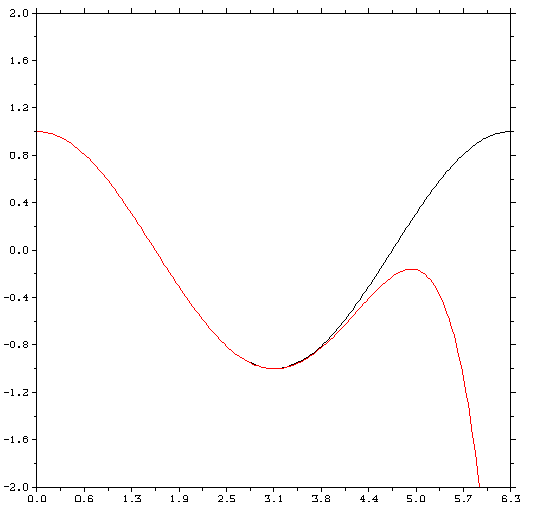
\includegraphics[width = \textwidth]{./doc/Figures/Taylor1.png}  \\
        \caption{Cosine (black) and Taylor expansion around $x_0 = 0$ with $N = 10$}
        \label{fig:Taylor1}
    \end{subfigure}
    \hspace{\fill}
    \begin{subfigure}[h]{0.4\textwidth}
        \centering
        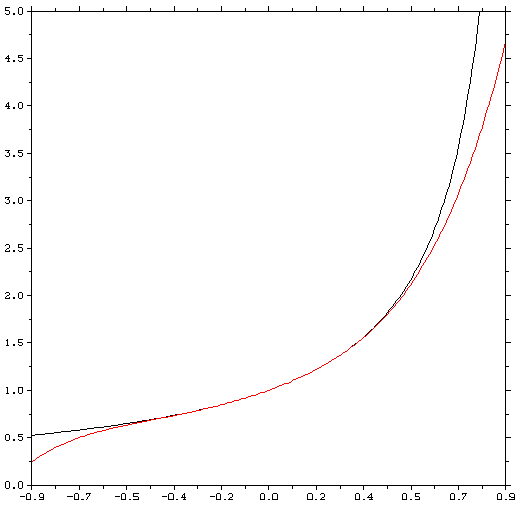
\includegraphics[width = \textwidth]{./doc/Figures/Taylor2.png}  \\
        \caption{Function $f(x) = \frac{1}{1-x}$ (black) and Taylor expansion around $x_0 = 0$ with $N = 5$}
        \label{fig:Taylor2}
    \end{subfigure}    

    \centering
    \begin{subfigure}[h]{0.4\textwidth}
        \centering
        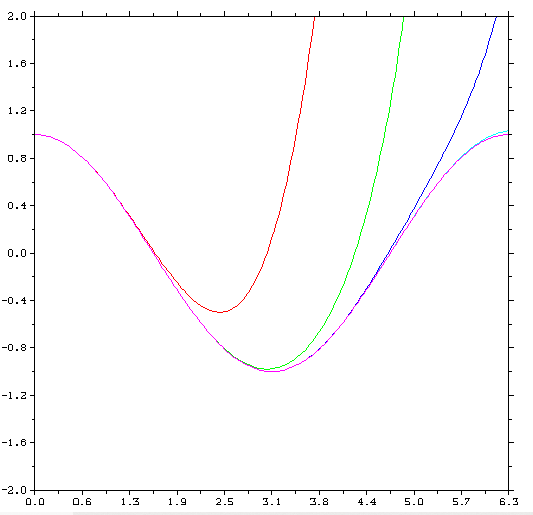
\includegraphics[width = \textwidth]{./doc/Figures/Taylor3.png}  \\
        \caption{Cosine (black) and different Taylor expansions around $x_0 = 0$ with $N = 1, 5, 9, 13, 17, 21$ and $25$}
        \label{fig:Taylor3}
    \end{subfigure}
    \caption{Different Taylor expansions for functions.}   \label{fig:Taylor}
\end{figure}


  
 
 \newpage 
 \subsection*{Python code} 
 The same functions are coded now with Python, notice that overloading both into one function called \texttt{Taylor} is performed in a different way.
 
 \vspace{0.5cm}
 \renewcommand{\home}{./Python/sources/Foundations/Calculus} 
 \lstpython
 \listings{\home/Taylor_expansions.py}{def Taylor}
 {exit}{Taylor_expansions.f90}
 
 \listings{\home/Taylor_expansions.py}{def Taylor_e}
 {Sigma}{Taylor_expansions.f90}
  
 \listings{\home/Taylor_expansions.py}{def Taylor_N}
 {Sigma}{Taylor_expansions.f90}
  
 
    
   
   \newpage 
   Try the same examples treated with Fortran in the Python project attached to this book:
      
   \vspace{0.5cm}
   \listings{\home/Examples/Series_expansion.py}{def Taylor_expansion_examples}
   {end}{Series_expansion.py}
   \lstfor
   
   
   
   
 % Taylor_expansion_examples
  
  
  
  
  
   
\newpage 
%___________________________________________________________________________________________________
\section{Parseval's identity} 

Let's consider a function $f(x)$ and its Fourier series expansion, whether expressed as a sines-cosines expansion:
\begin{equation} 
	f ( x)  =  \sum_{k=0} ^{\infty} \  \hat{a}_k  \ \cos\left(k x\right)  + \sum_{k=1} ^{\infty} \  \hat{b}_k  \sin\left(k x\right)
\end{equation} 	

or as a complex form:
\begin{equation} 
    f ( x)  =  \sum_{k=-\infty} ^{\infty}  \hat{c}_k  e^{ i k x }
\end{equation} 

Notice that for this expressions the function $f(x)$ is considered real-valued and periodic with period $T=2\pi$. As we know, the computer can not compute an infinite number of terms, we must truncate the series somewhere, let's say when $k = N-1$ so a total of $N$ terms are considered. Then, the expansion becomes:
\begin{equation} 
    f ( x)  =  \sum_{k=0} ^{N-1} \  \hat{a}_k  \ \cos\left(k x\right) + \sum_{k=1} ^{N-1} \  \hat{b}_k  \sin \left(k x\right)
\end{equation}

or in complex form, those $N$ terms becomes:
\begin{equation} 
    f ( x)  =  \sum_{k=-\frac{N}{2}} ^{\frac{N}{2}-1}  \hat{c}_k  e^{ i k x }
\end{equation} 

We can quickly revise the relation between the coefficients of the sines-cosines expansion and the coefficients of the complex series expansion:  

$$
\begin{cases}
    \hat{c}_k  =  \frac{1}{2} \ ( \ \hat{a}_k  - i \ \hat{b}_k \ ),  \quad k=1, \ldots, N/2.   \\
    \hat{c}_0  = \hat{a}_0   \\
    \hat{c}_{-k}  =  \overline{ \hat{c} } _{k}  , \quad k=1, \ldots, N/2. 
\end{cases}
$$

With that in mind, the Parseval's identity says:
\begin{equation} 
	\int _{-\pi} ^{\pi} f(x)^2 \ dx =  2 \pi  \sum_{k=-\infty} ^{\infty}  | \hat{c}_k | ^2       =  2 \pi \left(    | \hat{c}_0 |^2 + 2 \sum_{k=1} ^{\infty} |  \hat{c}_k  |^2 \right) 
\end{equation} 





A good example, related to previous chapters, is the following: consider the function $ f(x) = x \quad $ $ \forall x \in [-\pi, +\pi ) $ and extend it periodically to the right and to the left. Once $ f(x) $ is defined in this way, it can be approximated by a sine expansion: 
%\begin{equation} 
%	f ( x)  =  \sum_{k=1} ^{N/2} \   \hat{b}_k  \sin k x, 
%\end{equation} 
\begin{equation} 
	f ( x )  =  \sum_{k=1} ^{\infty} \   \hat{b}_k  \sin \left(  kx\right), 
\end{equation} 
where the coefficients $ \hat{b}_k $ are given by:
%\begin{equation} 
%	\hat{b}_k   = \frac{ (-1)^{k+1} }{ \pi k }, \qquad k=1, \ldots, N/2. 
%\end{equation} 
\begin{equation} 
    \hat{b}_k   = \frac{ 2 (-1)^{k+1} }{ k }, \qquad k=1, \ldots,\infty. 
\end{equation} 

Using the Parseval's identity with $f(x)$:
$$
\int_{-\pi}^{\pi}  x^2 dx  = \frac{2}{3} \pi^3 = 2\pi \left(   2\sum_{k=1}^{\infty}  \mid  -\frac{1}{2} i \hat{b}_k   \mid ^2  \right)
$$

and the following summation is obtained: 
%\begin{equation} 
%	\sum_{k=1} ^{\infty} \  \frac{1}{n^2}  \  = \frac{\pi^2}{6}
%\end{equation} 
\begin{equation} 
    \sum_{k=1} ^{\infty} \  \frac{1}{k^2}  \  = \frac{\pi^2}{6}
\end{equation}



